\section{Solving the recurrences}\label{chap:recurrenceAnalysis}

In Chapter~\ref{chap:noregen} we obtained the length of a fight in terms of the recurrence relations
\begin{align}\label{eq:complexRecurrence1}
	\L_h = \begin{cases}
        \frac{m+1}{m}\L_{h-1} - \frac{1}{m}\L_{h-m-1} &\quad \mbox{if } h > m+1\\
        \frac{m+1}{m}\L_{h-1} &\quad \mbox{if } h \leq m+1
    \end{cases}
\end{align}
and the initial condition $L_1 = \frac{m+1}{ma}$. The case $h \leq m+1$ is simply the recurrence relation for a geometric sequence. Therefore,
\begin{align}
    \overline{L}_h &= \frac{1}{a} {\left( \frac{m+1}{m} \right)}^h \quad \mbox{if } h \leq m+1.\label{eq:geomProgression}
\end{align}

The recurrence relation for the case $h > m+1$ is not as easy to bring in a non-recursive form. It is a linear recurrence of order $m$, the initial $m$ elements of which are given by eq\ref{eq:geomProgression}. Inspired by the geometric progression, we define
\begin{align}
	r &= \frac{m+1}{m} \quad \mbox{and } \quad p = \frac{-1}{m+1}
\end{align}
and restate the recurrence relation and its initial condition a bit more neatly.
\begin{align}\label{eq:complexRecurrence2}
	\L_h = \begin{cases}
        r\left(\L_{h-1} - p\L_{h-m-1}\right) &\quad \mbox{if } h \leq m+1\\
        \frac{1}{a}r^h &\quad \mbox{if } h > m+1
    \end{cases}
\end{align}

This recurrence is perhaps most effectively approached with generating functions. The ordinary generating function of the number sequence $\L_h$ is a the function $g(z)$ whose power series expansion has $\L_h$ as coefficients.
\begin{align}
    g(z) = \sum_{h=1}^{\infty} \L_h z^h
\end{align}
Using the generating function formulation the recurrence (eq\ref{eq:complexRecurrence2}) translates into an algebraic equation for $g(z)$. Usually, for linear recurrences one would save some work by directly writing down the charasteristic polynomial $1 - rz - rpz^{m+1}$ and considering the initial values. For completeness, the full derivation will be given. It is straightforward but quite tedious, so feel free to skip ahead to the result (eq\ref{eq:ogf}).
\begin{align}
    g(z) &= \sum_{h=1}^{m+1} \L_h z^h + \sum_{h=m+2}^{\infty} \L_h z^h\nonumber\\
         &= \sum_{h=1}^{m+1} \L_h z^h + \sum_{h=m+2}^{\infty} r\left(\overline{L}_{h-1} + p\overline{L}_{h-m-1}\right)z^h\nonumber\\
         &= \sum_{h=1}^{m+1} \L_h z^h + rz\sum_{h-1=m+1}^{\infty}\overline{L}_{h-1}z^{h-1} + rpz^{m+1}\sum_{h-m-1=1}^{\infty}\overline{L}_{h-m-1}z^{h-m-1}\nonumber\\
         &= \sum_{h=1}^{m+1} \L_h z^h + rz\sum_{h=m+1}^{\infty}\overline{L}_{h}z^{h} + rpz^{m+1}\sum_{h=1}^{\infty}\overline{L}_{h}z^{h}\nonumber\\
         &= \sum_{h=1}^{m} \L_h z^h + \L_{m+1} z^{m+1} + rz\left(- \sum_{h=1}^{m}\overline{L}_{h}z^{h} + \sum_{h=1}^{\infty}\overline{L}_{h}z^{h}\right) + rpz^{m+1}g(z)\nonumber\\
         &= (1 - rz)\sum_{h=1}^{m} \L_h z^h + \L_{m+1} z^{m+1} + \left(rz + rpz^{m+1}\right)g(z)
\end{align}
Now, moving all terms containing $g(z)$ to the left and substituting the values for $\L_h$ from eq\ref{eq:geomProgression} gives
\begin{align}
    (1 - rz - rpz^{m+1})g(z) &= \frac{1}{a}\left({(rz)}^{m+1} + (1 - rz)\sum_{h=1}^{m} {(rz)}^h\right)\label{eq:ogfderiv1}
\end{align}
The partial sum on the right is the $m$ first terms of a geometric series which has the following closed form expression.
\begin{align*}
    \sum_{h=1}^{m} {(rz)}^h = rz\frac{1 - {(rz)}^m}{1-rz}
\end{align*}
Plugging it back to eq\ref{eq:ogfderiv1} to gives
\begin{align}
    (1 - rz - rpz^{m+1})g(z) &= \frac{1}{a}\left({(rz)}^{m+1} + rz\left(1 - {(rz)}^m\right)\right)\nonumber
                            = \frac{1}{a}rz\nonumber
                            = \L_1 z\nonumber\\
    \implies           g(z) &= \frac{\L_1 z}{1 - rz - rpz^{m+1}}\label{eq:ogf}.
\end{align}

To read off the explicit formula for $\L_h$ the generating function must be expanded back into a power series. This is possible by noticing that $g(z)$ is an infinite geometric sum with $rz(1 - pz^m)$ as its coefficient.
\begin{align}
    g(z) &= \frac{\L_1 z}{1 - rz\left(1 + pz^{m}\right)}\nonumber
    = \L_1 z\sum_{n=0}^\infty {(rz(1 + pz^m))}^n\nonumber
    = \frac{1}{a} \sum_{n=0}^\infty {(rz)}^{n+1}{(1 + pz^m)}^n
\end{align}
Then, we expand the $n$th order binomial term using the binomial theorem.
\begin{align}
    g(z) &= \frac{1}{a} \sum_{n=0}^\infty {(rz)}^{n+1}\sum_{i=0}^{n} {(pz^m)}^i {n \choose i}\nonumber\\
         &= \sum_{n=0}^\infty \frac{1}{a}\sum_{i=0}^{n} r^{n+1} p^i {n \choose i}z^{mi+n+1}\label{eq:ogf2}.
\end{align}
$\L_h$ is now the coefficient of the term $z^h$. Looking at the exponent of $z$ in eq\ref{eq:ogf2} we see that for the coefficient of interest the indices $i$ and $n$ must satisfy $h=mi+n+1$. For each $i$ there is exactly one valid $n$, namely $n = h-mi-1$.
Therefore, the coefficient of the $h$th order term in the series expansion of $g(z)$ is
\begin{align}
    \L_h &= \frac{1}{a}\sum_{i \in \mathcal{I}} r^{h-mi} p^i {h-mi-1 \choose i} \nonumber
\end{align}
where $\mathcal{I}$ is the set of indices $i$ such that
\begin{align*}
    0 \leq i \leq n = h-mi-1
    \iff (m+1)i \leq h-1
    \iff i \leq \frac{h-1}{m+1}.
\end{align*}
Since $i$ must also be an integer the index set becomes $\mathcal{I} = \left\{0,1,\ldots,\left\lfloor{\frac{h-1}{m+1}}\right\rfloor\right\}$. Expressing the constants $r$ and $p$ explicitly, the solution to the recursion problem (eq\ref{eq:complexRecurrence2}) can be written as
\begin{align}
    \L_h &= \frac{1}{a}\sum_{i=0}^{\left\lfloor{\frac{h-1}{m+1}}\right\rfloor} {\left(\frac{m+1}{m}\right)}^{h-mi} {\left(\frac{-1}{m+1}\right)}^i {h-mi-1 \choose i}.\label{eq:explicitL}
\end{align}
Naturally this can also be proven to satisfy the recursion using induction (see Appendix~\ref{sect:genLProof}). With this result the damage dealt per hit is simply $h/\L_h$ and the damage per second can be obtained from it by dividing with the attack interval $T_A$.

Eq\ref{eq:explicitL} can be annoying to work with, especially for large $h$, so an approximation for the case $h \gg m$ is needed. Intuitively the length of a fight should have linear dependency on hitpoints as $h \rightarrow \infty$. This is because on average one can expect each hit to do $am/2$ damage and therefore it should take approximately $2h/am$ hits to kill an enemy with $h$ hitpoints. Due to overkill however, the last hit will do slightly less than $am/2$ damage on average introducing a constant correction term to this linear approximation.
The average length of a fight with no regeneration has the following asymptotic behaviour (derivation not shown here).
\begin{align}\label{eq:asymptoticAppr}
\L_h \sim \frac{2}{ma}\left(h + \frac{m-1}{3}\right)
\end{align}
The correctness of both the results was validated by comparing them to a computer simulation. The comparison is illustrated in figure~2.
\begin{figure}[t]\label{fig:apprComparison}
    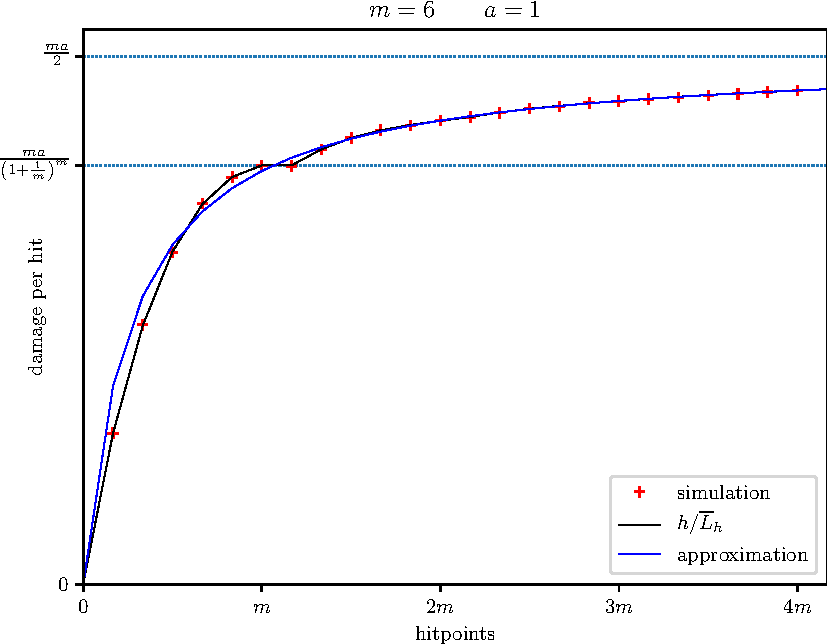
\includegraphics[scale=1.1]{dph-appr-m6.pdf}
    \caption{Comparison of damage per hit (DPH) calculated using the explicit formula (eq\ref{eq:explicitL}), asymptotic approximation (eq\ref{eq:asymptoticAppr}) and a simulation. The simulation was written using the damage calculation mechanics described in Chapter~\ref{chap:fightDef}. For each datapoint $10^{5}$ fights were simulated and their average lengths calculated.}
\end{figure}
